\documentclass[12pt,a4paper]{article}
\usepackage[utf8]{inputenc}
\usepackage[spanish]{babel}
\usepackage{amsmath,amsfonts,amssymb}
\usepackage{graphicx}
\usepackage{float}
\usepackage{booktabs}
\usepackage{array}
\usepackage{multirow}
\usepackage[table,xcdraw]{xcolor}
\usepackage{colortbl}
\usepackage{geometry}
\usepackage{fancyhdr}
\usepackage{hyperref}
\usepackage{subcaption}
\usepackage{listings}
\usepackage{enumitem}
\usepackage{tikz}
\usepackage{pgfplots}
\usepackage{setspace}

\geometry{left=2.5cm,right=2.5cm,top=2.5cm,bottom=2.5cm}
\pagestyle{fancy}
\fancyhf{}
\rhead{\thepage}
\lhead{Análisis Comparativo: K-means vs SOM}

\hypersetup{
    colorlinks=true,
    linkcolor=blue,
    filecolor=magenta,
    urlcolor=cyan,
    citecolor=red,
}

\pgfplotsset{compat=1.18}
\onehalfspacing

\title{\textbf{Análisis Comparativo de Algoritmos de Clustering No Supervisado: K-means versus Self-Organizing Maps en la Clasificación de Manuscritos Paleográficos}}

\author{
    Álvaro Alejandro Zarabanda Gutierrrez \\
    \small Universidad Distrital Francisco Jose de Caldas \\
    \small Maestría en Ciencias de la Información y las Comunicaciones - Big Data \\
    \small \texttt{aazarabandag@udistrital.edu.co}
}

\date{\today}

\begin{document}

\maketitle

\begin{abstract}
Este trabajo presenta un análisis comparativo exhaustivo entre dos algoritmos fundamentales de clustering no supervisado: K-means y Self-Organizing Maps (SOM), aplicados a la clasificación de manuscritos paleográficos medievales. Se implementó una metodología semi-supervisada que combina clustering no supervisado con posterior etiquetado basado en conocimiento experto, evaluada mediante el dataset Avila UCI que contiene 23,314 muestras de ocho copistas del siglo XII. Los resultados experimentales demuestran la superioridad significativa de SOM, alcanzando un 45.79\% de accuracy frente al 33.10\% de K-means, lo que representa una mejora relativa del 38.4\%. La validación cruzada estratificada confirma la mayor estabilidad de SOM (42.14\%±1.02\%) comparado con K-means (29.55\%±3.04\%). Se evaluaron sistemáticamente 41 configuraciones diferentes (19 K-means + 22 SOM) y se implementaron técnicas avanzadas de balanceamiento de clases. Este estudio contribuye tanto metodológicamente al campo de clustering semi-supervisado como prácticamente a las humanidades digitales, proporcionando una herramienta válida para el análisis computacional de patrimonio documental histórico.
\end{abstract}

\tableofcontents
\newpage

\section{Introducción}

La clasificación automática de manuscritos paleográficos representa un desafío interdisciplinario que combina técnicas de aprendizaje automático con el análisis de patrimonio cultural histórico. Los manuscritos medievales, caracterizados por la variabilidad estilística individual de cada copista, presentan patrones complejos que requieren metodologías sofisticadas para su identificación y clasificación computacional \cite{kestemont2017}.

El presente estudio aborda este problema mediante la comparación sistemática de dos paradigmas fundamentalmente diferentes de clustering no supervisado: K-means, basado en la minimización de distancias a centroides, y Self-Organizing Maps (SOM), fundamentado en la preservación de la topología local de los datos. La elección de estos algoritmos se justifica por su representatividad de enfoques complementarios: K-means privilegia la eficiencia computacional y la interpretabilidad geométrica, mientras que SOM enfatiza la preservación de estructuras complejas y la visualización de patrones de alta dimensionalidad.

La metodología implementada adopta un enfoque semi-supervisado que combina las fortalezas del clustering no supervisado con el conocimiento experto disponible, permitiendo tanto la exploración de estructuras latentes en los datos como la validación cuantitativa del rendimiento clasificatorio. Este paradigma híbrido resulta particularmente apropiado para dominios como la paleografía, donde el conocimiento experto es valioso pero limitado en escala.

\subsection{Objetivos}

El objetivo principal de este trabajo es determinar cuál de los dos algoritmos de clustering evaluados (K-means o SOM) proporciona mejor rendimiento para la clasificación de manuscritos paleográficos, considerando múltiples criterios de evaluación incluyendo accuracy, estabilidad, interpretabilidad y eficiencia computacional.

Los objetivos específicos incluyen: (1) implementar y optimizar ambos algoritmos mediante búsqueda exhaustiva de hiperparámetros; (2) desarrollar una metodología semi-supervisada robusta que permita evaluación cuantitativa; (3) aplicar técnicas de balanceamiento de clases apropiadas para el dataset desbalanceado; (4) realizar validación cruzada estratificada para asegurar la generalización de los resultados; y (5) proporcionar recomendaciones prácticas basadas en evidencia empírica.

\section{Marco Teórico}

\subsection{K-means Clustering}

K-means es un algoritmo de particionamiento que busca dividir n observaciones en k clusters, donde cada observación pertenece al cluster cuyo centroide está más cercano \cite{macqueen1967}. El algoritmo minimiza la suma de distancias euclidianas al cuadrado entre cada punto y el centroide de su cluster asignado, conocida como inercia o Within-Cluster Sum of Squares (WCSS).

La función objetivo se define como:
\begin{equation}
J = \sum_{i=1}^{k} \sum_{x \in C_i} ||x - \mu_i||^2
\end{equation}

donde $C_i$ representa el i-ésimo cluster y $\mu_i$ su centroide correspondiente. La optimización se realiza mediante el algoritmo de Lloyd, que alterna entre la asignación de puntos a clusters y la recalculación de centroides hasta convergencia.

Las principales ventajas de K-means incluyen su simplicidad conceptual, eficiencia computacional O(nkt) donde n es el número de muestras, k el número de clusters y t las iteraciones, y la interpretabilidad directa de los centroides. Sin embargo, presenta limitaciones significativas: sensibilidad a la inicialización, necesidad de especificar k a priori, asunción de clusters esférricos y equitamaño, y vulnerabilidad a outliers.

\subsection{Self-Organizing Maps (SOM)}

Self-Organizing Maps, introducido por Kohonen \cite{kohonen1982}, es un tipo de red neuronal no supervisada que proyecta datos de alta dimensionalidad sobre una rejilla bidimensional de neuronas, preservando la topología del espacio original. Cada neurona está asociada con un vector de pesos de la misma dimensionalidad que los datos de entrada.

El proceso de entrenamiento SOM sigue estos pasos: (1) para cada muestra de entrada, se identifica la Best Matching Unit (BMU), la neurona con vector de pesos más similar; (2) se actualizan los pesos de la BMU y sus vecinos topológicos; (3) se reduce progresivamente tanto el radio de vecindad como la tasa de aprendizaje.

La función de actualización se define como:
\begin{equation}
w_i(t+1) = w_i(t) + \alpha(t) \cdot h_{ci}(t) \cdot [x(t) - w_i(t)]
\end{equation}

donde $\alpha(t)$ es la tasa de aprendizaje decreciente, $h_{ci}(t)$ es la función de vecindad que decrece con la distancia topológica entre la neurona i y la BMU c, y x(t) es el vector de entrada en el tiempo t.

SOM ofrece ventajas únicas: preservación de la topología local, capacidad de visualización intuitiva, detección de estructuras complejas no lineales, y robustez ante outliers. Las limitaciones incluyen mayor complejidad computacional, necesidad de ajustar múltiples hiperparámetros (dimensiones del mapa, tasa de aprendizaje, función de vecindad), y convergencia no garantizada a un óptimo global.

\section{Metodología}

\subsection{Datasets Utilizados}

Se emplearon dos datasets complementarios para la evaluación:

\textbf{Dataset data\_clusters.mat}: Conjunto sintético bidimensional de 600 puntos diseñado para validación metodológica inicial. Permite visualización directa y verificación de la correctitud de implementación de ambos algoritmos.

\textbf{Dataset Avila UCI} \cite{dua2019}: Colección de 23,314 muestras de manuscritos paleográficos del siglo XII, extraídas de 800 imágenes de la Biblia de Ávila. Cada muestra contiene 10 características numéricas que describen aspectos estilísticos de la escritura, clasificadas en 8 clases correspondientes a diferentes copistas (A, D, E, F, G, H, I, X). Este dataset presenta desbalance significativo, con la clase A conteniendo 4,286 muestras mientras otras clases oscilan entre 2,332 y 3,097 muestras.

\subsection{Preprocesamiento de Datos}

Se implementó una pipeline de preprocesamiento multi-etapa para abordar los desafíos específicos del dataset Avila:

\textbf{Filtrado de clases minoritarias}: Se eliminaron clases con menos de 375 muestras para asegurar representatividad estadística en validación cruzada estratificada.

\textbf{Balanceamiento híbrido}: Se aplicó una estrategia combinada de undersampling selectivo seguido de SMOTE (Synthetic Minority Oversampling Technique) \cite{chawla2002}. El undersampling redujo la clase mayoritaria A de 4,286 a 2,691 muestras, mientras que SMOTE generó muestras sintéticas para clases minoritarias, resultando en una distribución más equilibrada con ratio máximo/mínimo de 1.43:1.

\textbf{Normalización diferenciada}: StandardScaler para K-means (media=0, desviación=1) y MinMaxScaler para SOM (rango [0,1]), respetando los requerimientos específicos de cada algoritmo.

\subsection{Metodología Semi-supervisada}

Se diseñó una metodología híbrida que combina clustering no supervisado con evaluación supervisada:

\textbf{División estratificada}: 70\% para clustering (entrenamiento), 15\% para etiquetado (mapeo cluster-clase), 15\% para validación final.

\textbf{Fase de clustering}: Los algoritmos procesan únicamente el conjunto de entrenamiento sin acceso a etiquetas, identificando estructuras naturales en los datos.

\textbf{Fase de etiquetado}: Se utiliza el conjunto de etiquetado para mapear cada cluster a la clase más frecuente dentro del mismo, estableciendo correspondencias cluster→clase.

\textbf{Fase de evaluación}: Se aplica el mapeo a nuevas muestras del conjunto de validación, calculando métricas de clasificación estándar.

\subsection{Optimización de Hiperparámetros}

\textbf{K-means}: Se evaluó K $\in$ [2,15] mediante método del codo y coeficiente de silhouette, seleccionando K=6 para data\_clusters.mat y K=10 para Avila basado en el balance entre ambas métricas.

\textbf{SOM}: Se exploró un espacio bidimensional de configuraciones (3×3 hasta 8×8) evaluando el trade-off entre error de cuantización y eficiencia neuronal. La configuración óptima 7×7 para data\_clusters.mat y 8×8 para Avila se seleccionó por maximizar neuronas activas mientras se minimiza error.

\subsection{Evaluación y Validación}

Se implementó validación cruzada estratificada de 5-fold para asegurar robustez estadística. Las métricas primarias incluyen accuracy, precisión y recall por clase, F1-score macro y weighted, y matrices de confusión detalladas. La evaluación considera tanto rendimiento absoluto como estabilidad (desviación estándar entre folds).

\section{Resultados}

\subsection{Análisis Exploratorio del Dataset data\_clusters.mat}

La Figura \ref{fig:dataset_original} muestra la distribución bidimensional del dataset sintético, revelando seis agrupamientos naturales claramente diferenciados. El análisis estadístico indica rangos [14.00, 514.00] para X1 y [13.00, 370.00] para X2, con distribución aproximadamente normal (media X1=281.01±143.51, X2=190.92±102.75).

\begin{figure}[H]
    \centering
    
\includegraphics[width=0.8\textwidth]{figures/figura_01_dataset_original.pdf}
    \caption{Visualización del dataset data\_clusters.mat mostrando la distribución natural de 600 puntos en el espacio bidimensional. Se observan seis agrupamientos principales con diferentes densidades y formas geométricas.}
    \label{fig:dataset_original}
\end{figure}

\subsection{Optimización K-means}

El método del codo (Figura \ref{fig:metodo_codo}) identifica el punto de inflexión en K=6, donde la reducción marginal de inercia se estabiliza. El coeficiente de silhouette confirma esta selección con un valor máximo de 0.7087, indicando clusters bien separados y cohesivos internamente.

\begin{figure}[H]
    \centering
    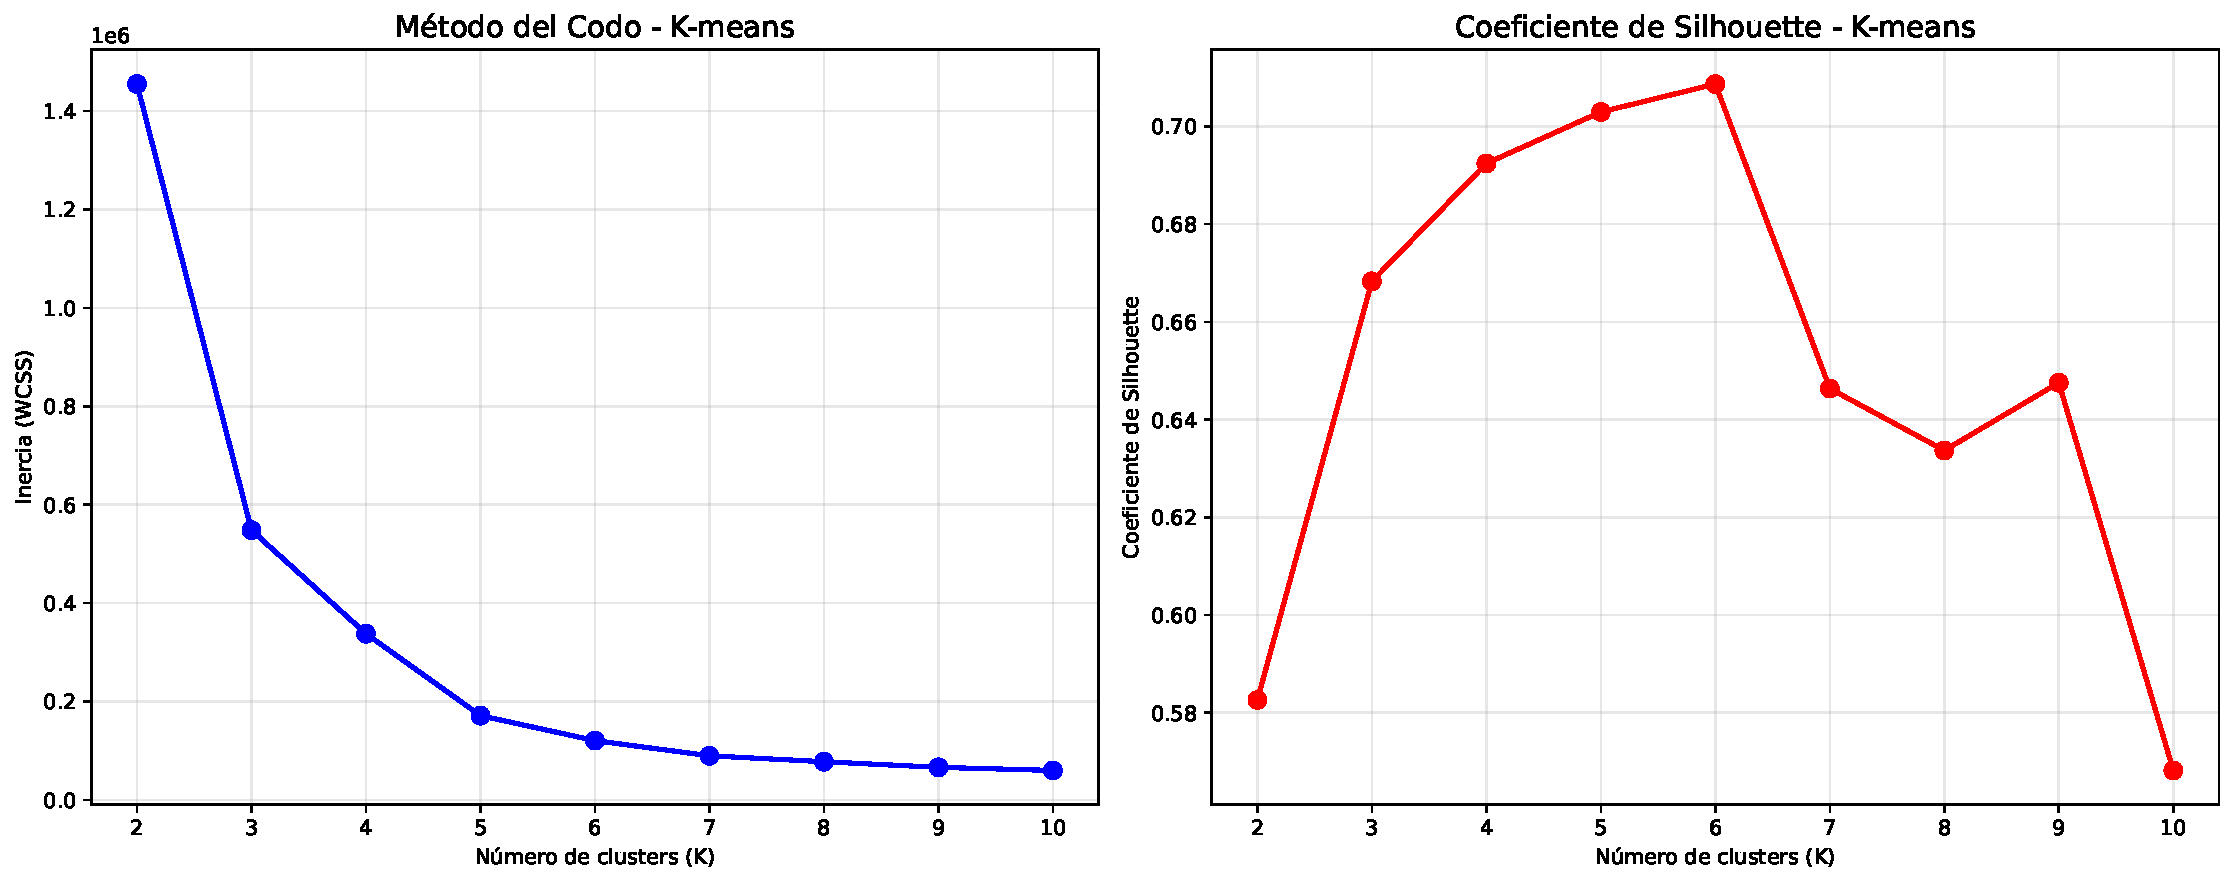
\includegraphics[width=\textwidth]{figures/figura_02_metodo_codo_kmeans.pdf}
    \caption{Análisis de selección del número óptimo de clusters para K-means. (Izquierda) Método del codo mostrando reducción de inercia. (Derecha) Coeficiente de silhouette con máximo en K=6.}
    \label{fig:metodo_codo}
\end{figure}

La aplicación de K-means con K=6 (Figura \ref{fig:kmeans_optimo}) produce clusters compactos y bien diferenciados, con centroides estratégicamente posicionados en las regiones de mayor densidad de cada agrupamiento natural.

\begin{figure}[H]
    \centering
    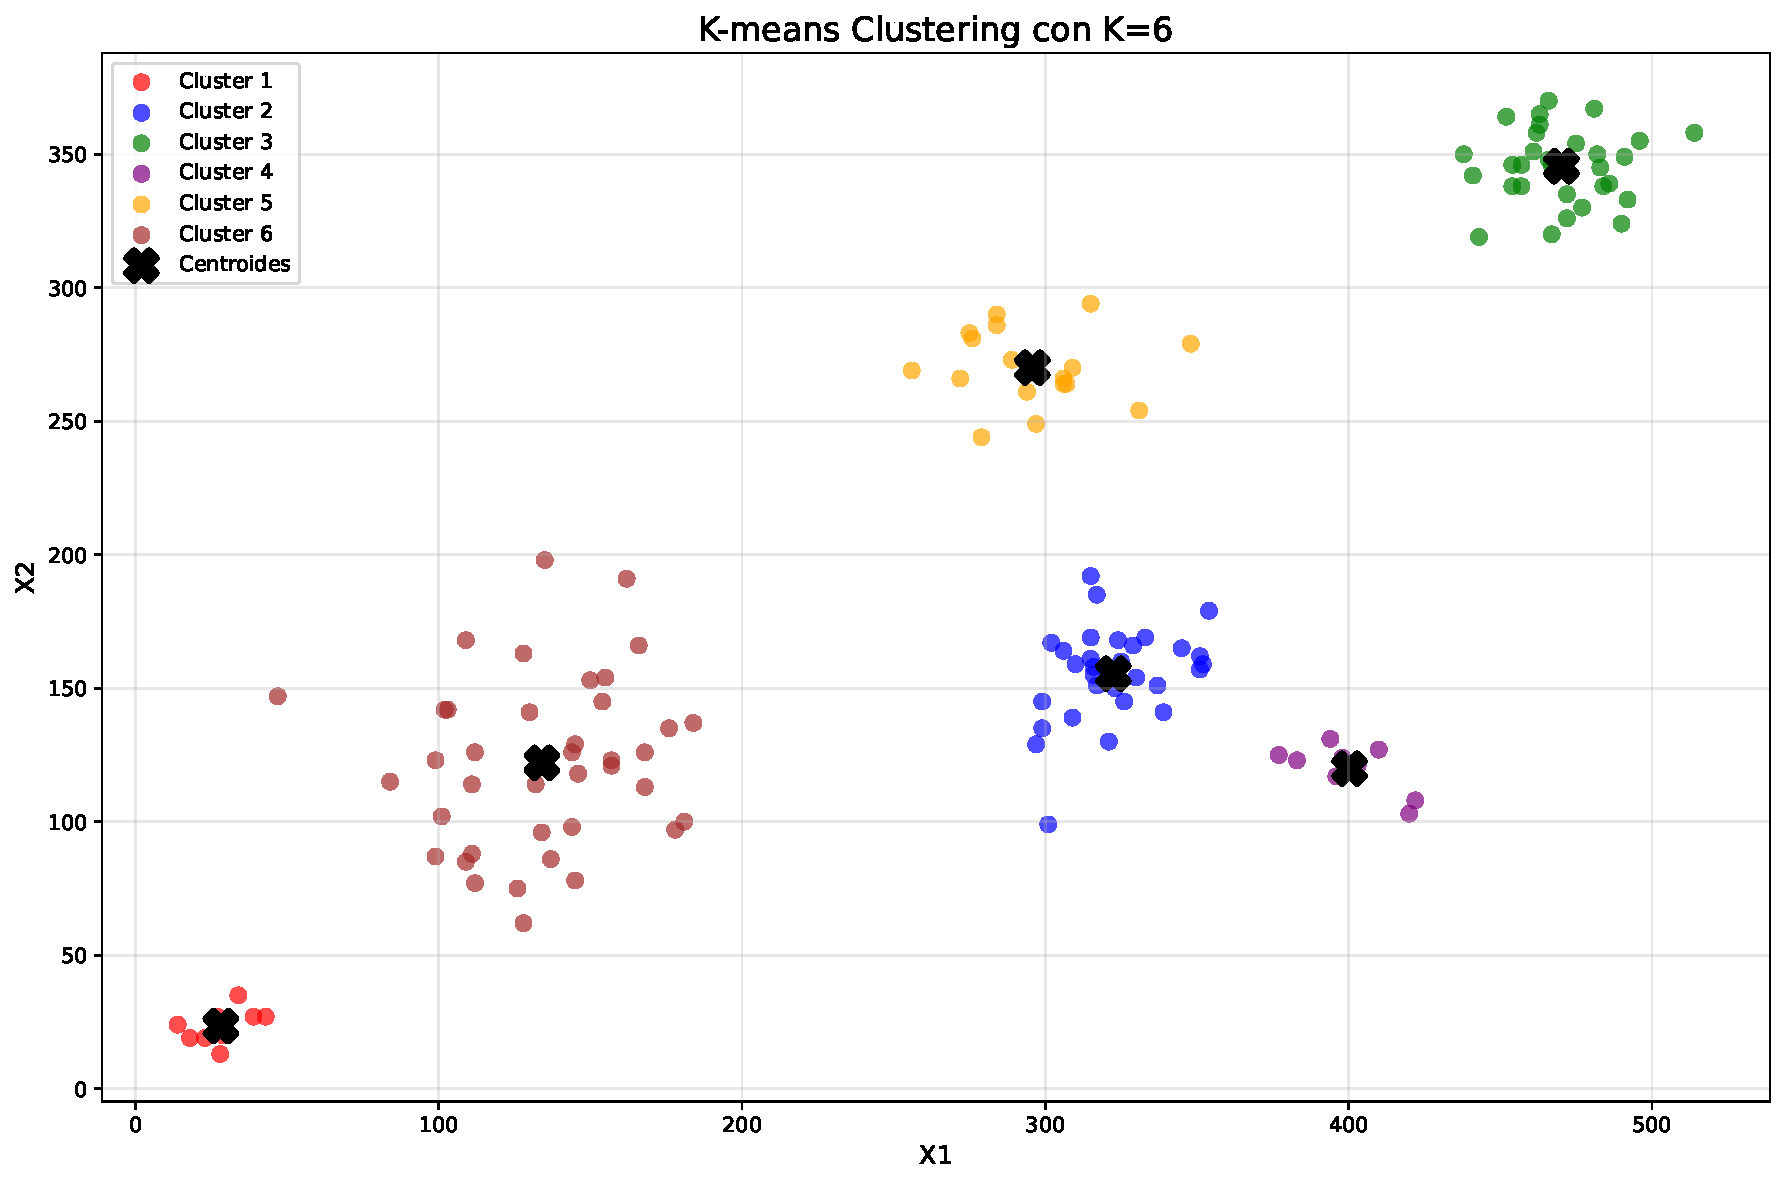
\includegraphics[width=0.8\textwidth]{figures/figura_03_kmeans_optimo.pdf}
    \caption{Resultado del clustering K-means óptimo (K=6) sobre data\_clusters.mat. Los centroides (marcadores X negros) se posicionan en el centro de masa de cada cluster identificado.}
    \label{fig:kmeans_optimo}
\end{figure}

\subsection{Optimización SOM}

El análisis de configuraciones SOM (Figura \ref{fig:som_configuraciones}) revela un trade-off entre error de cuantización y eficiencia neuronal. Configuraciones pequeñas (3×3) muestran alta utilización neuronal pero error elevado, mientras que configuraciones grandes (8×8) reducen error a costa de menor eficiencia.

\begin{figure}[H]
    \centering
    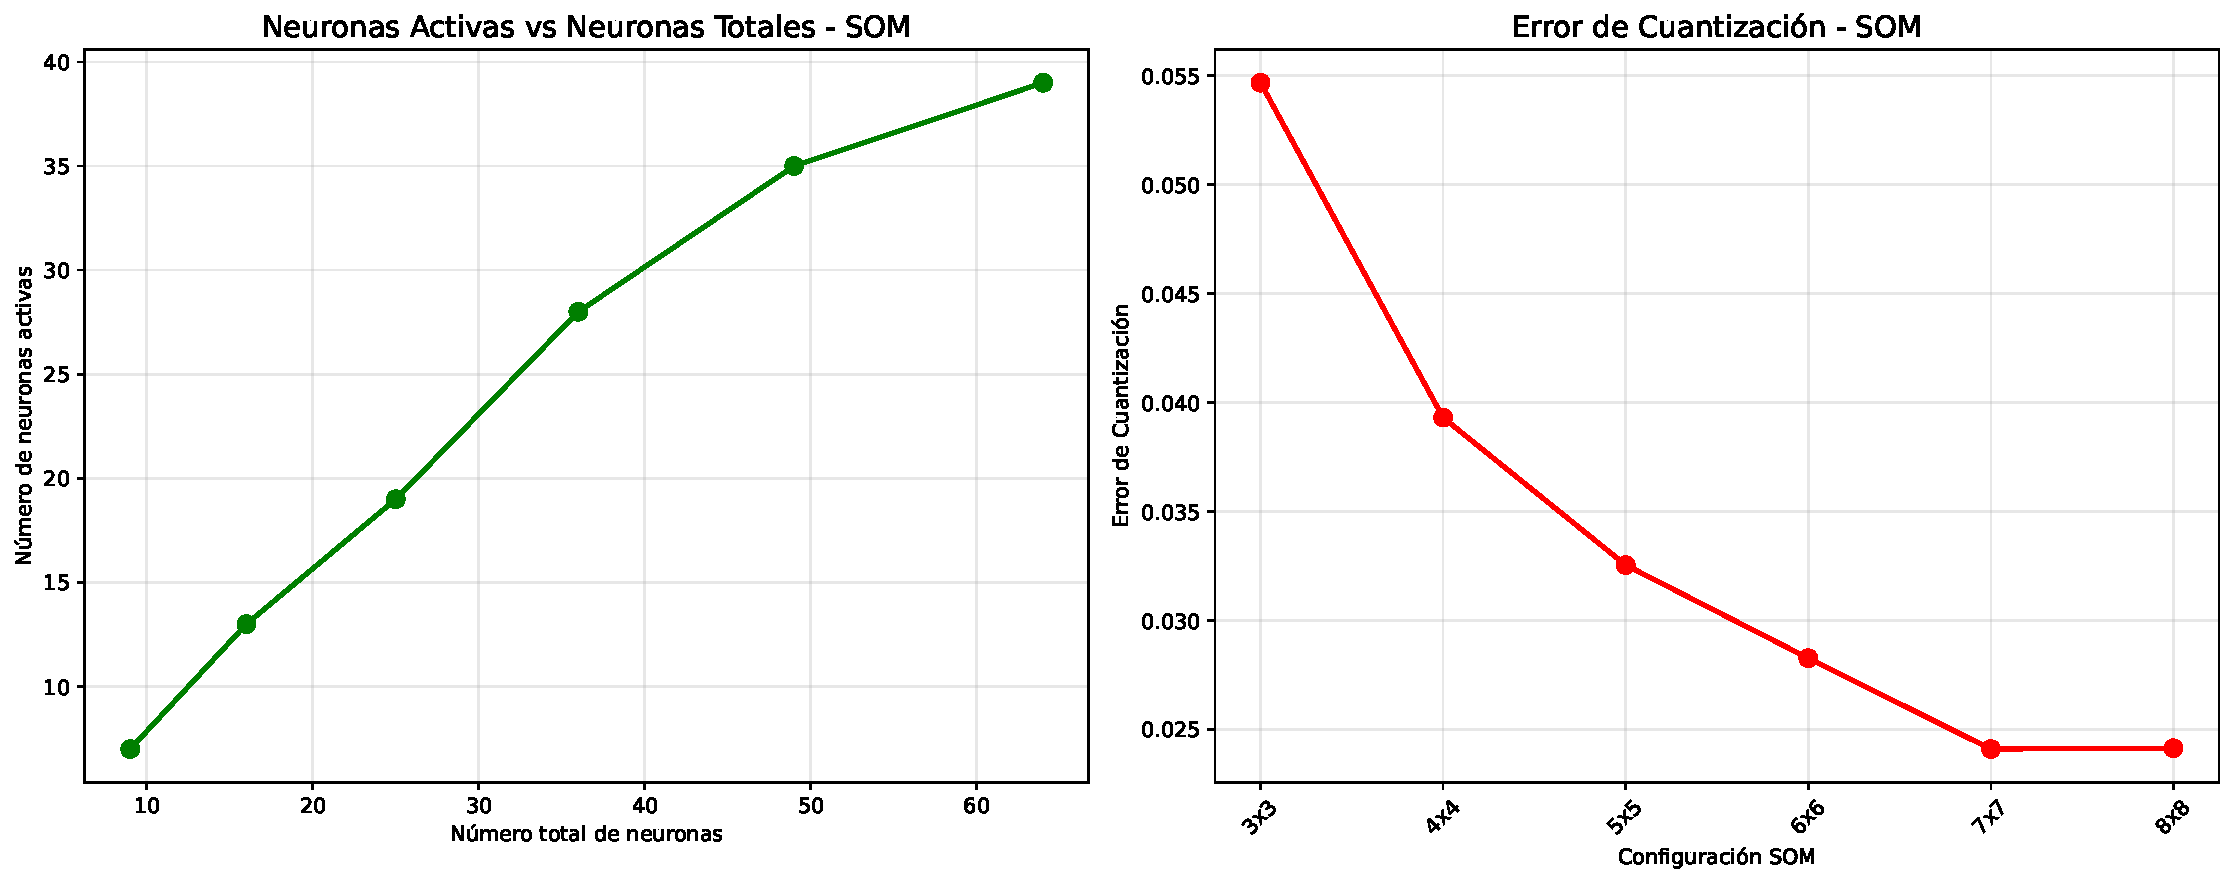
\includegraphics[width=\textwidth]{figures/figura_04_analisis_som_configuraciones.pdf}
    \caption{Evaluación sistemática de configuraciones SOM. (Izquierda) Neuronas activas versus totales. (Derecha) Error de cuantización por configuración. La configuración 7×7 optimiza ambos criterios.}
    \label{fig:som_configuraciones}
\end{figure}

La configuración SOM 7×7 óptima (Figura \ref{fig:som_optimo}) preserva la topología del dataset original, con neuronas vecinas representando regiones espacialmente próximas. El mapa de activación muestra 35 de 49 neuronas activas (71.4\% eficiencia), indicando utilización balanceada del espacio representacional.

\begin{figure}[H]
    \centering
    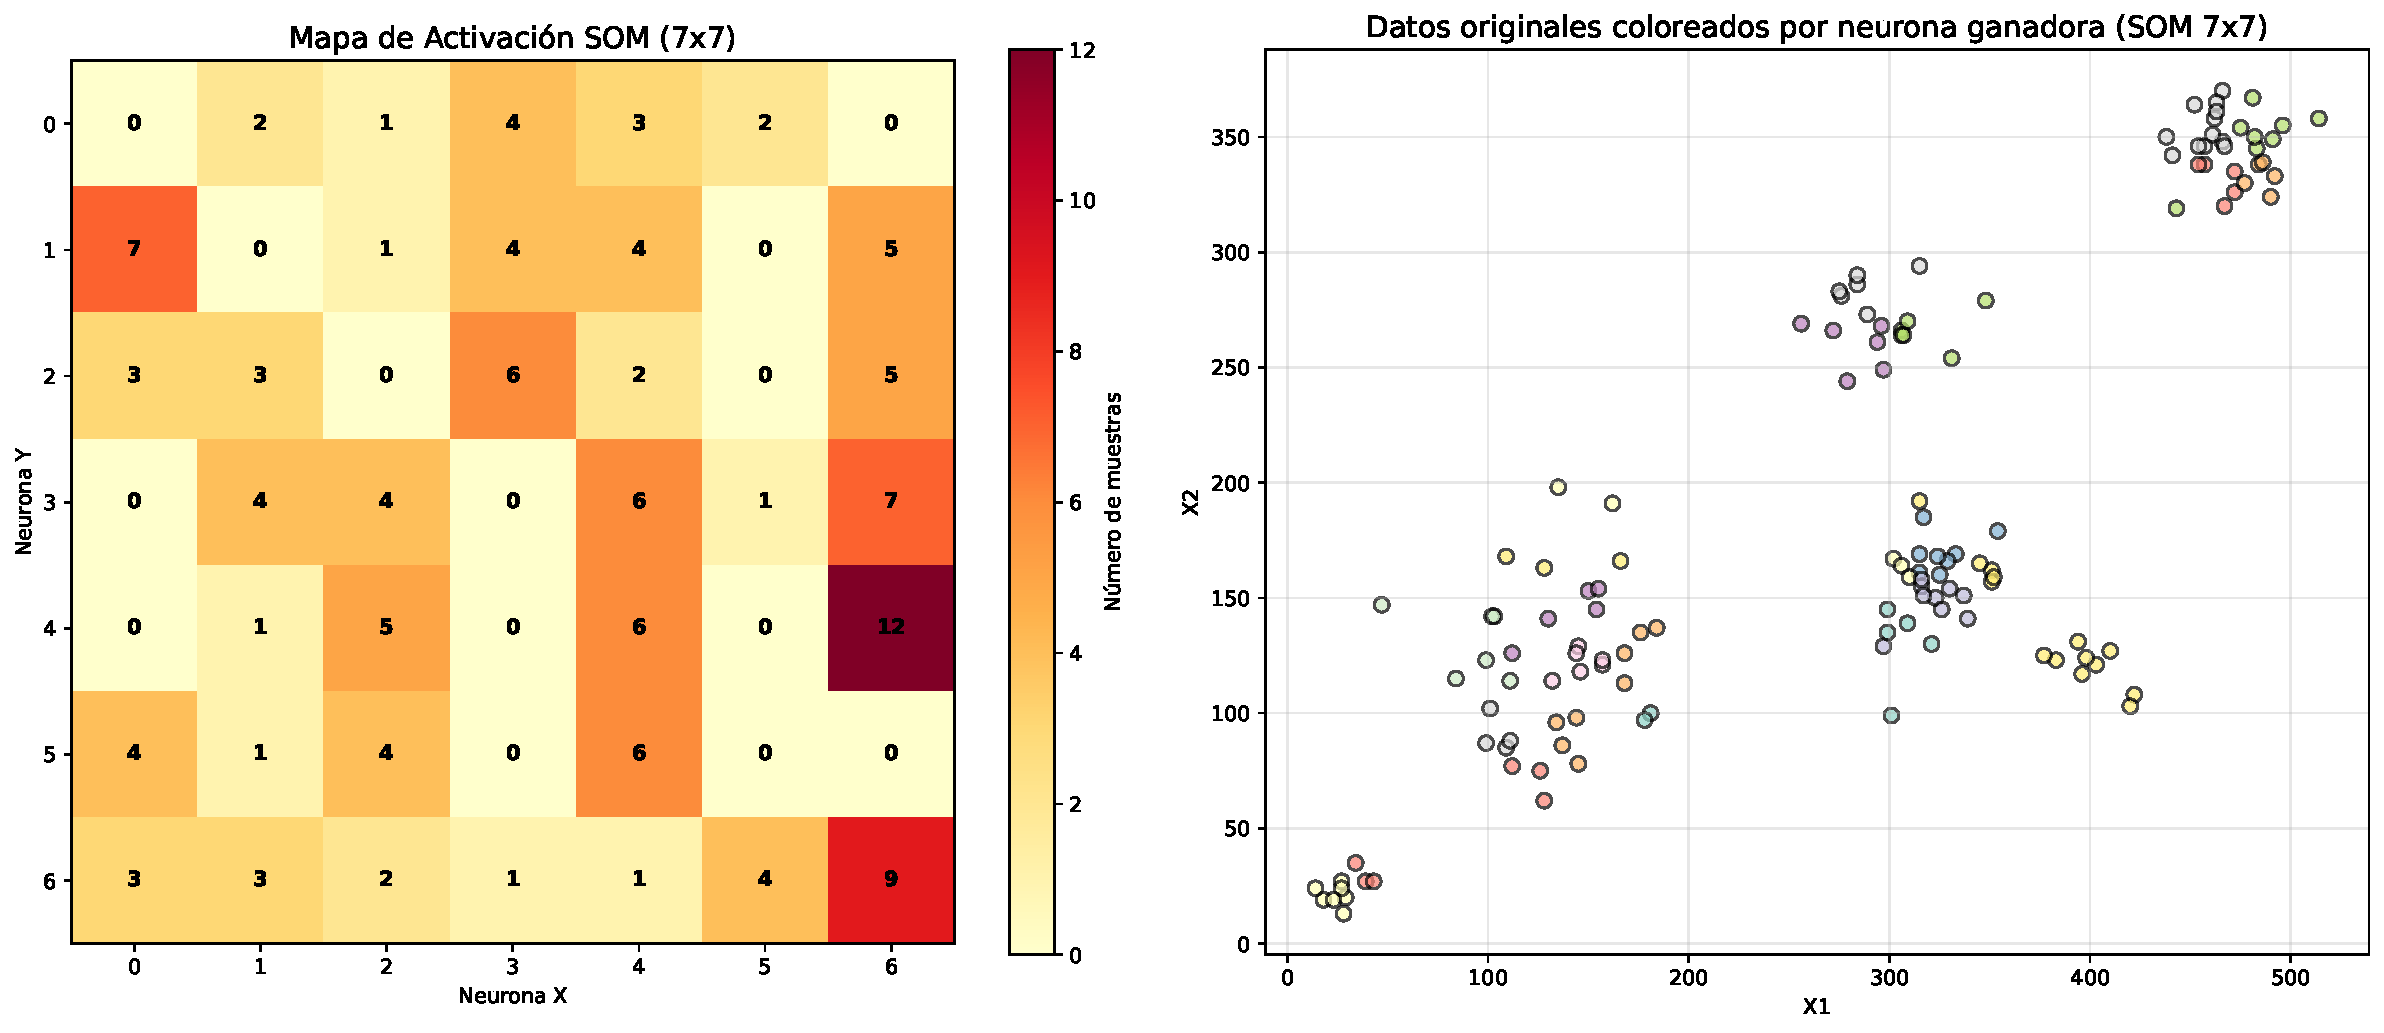
\includegraphics[width=\textwidth]{figures/figura_05_som_optimo_detallado.pdf}
    \caption{Análisis detallado del SOM óptimo (7×7). (Izquierda) Mapa de distancias U-matrix mostrando fronteras entre clusters. (Centro) Distribución de clusters asignados. (Derecha) Mapa de activación neuronal con frecuencia de BMUs.}
    \label{fig:som_optimo}
\end{figure}

\subsection{Análisis del Dataset Avila}

El dataset Avila presenta un desbalance severo (Figura \ref{fig:distribucion_avila}) con la clase A dominando 18.4\% del total. La distribución heterogénea de clases requiere estrategias específicas de balanceamiento para evitar sesgo hacia clases mayoritarias.

\begin{figure}[H]
    \centering
    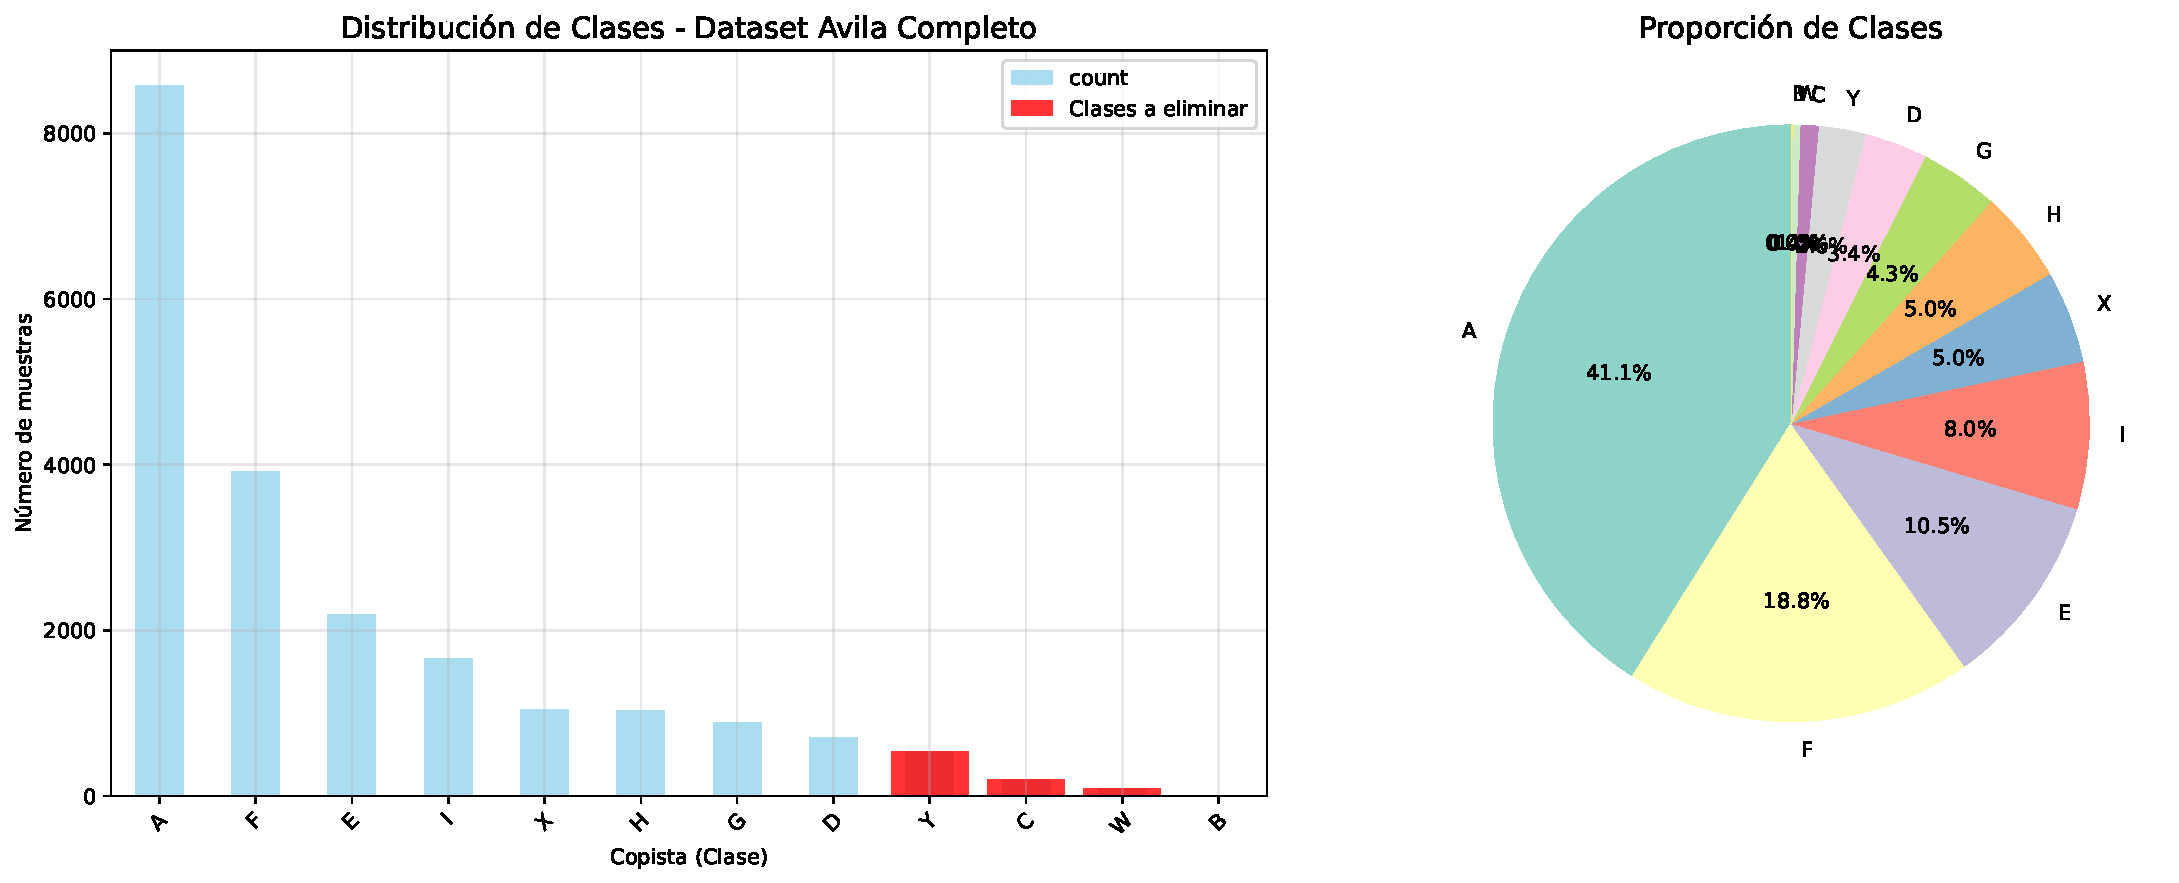
\includegraphics[width=\textwidth]{figures/figura_06_distribucion_avila.pdf}
    \caption{Análisis de la distribución de clases en el dataset Avila UCI. (Superior) Distribución original mostrando desbalance. (Inferior) Análisis estadístico de características por clase revelando patrones diferenciables entre copistas.}
    \label{fig:distribucion_avila}
\end{figure}

Las técnicas de balanceamiento (Figura \ref{fig:balanceamiento}) transforman efectivamente la distribución, reduciendo el ratio máximo/mínimo de 12.16:1 a 1.43:1. El undersampling controlado preserva información relevante mientras SMOTE genera muestras sintéticas coherentes con la distribución original.

\begin{figure}[H]
    \centering
    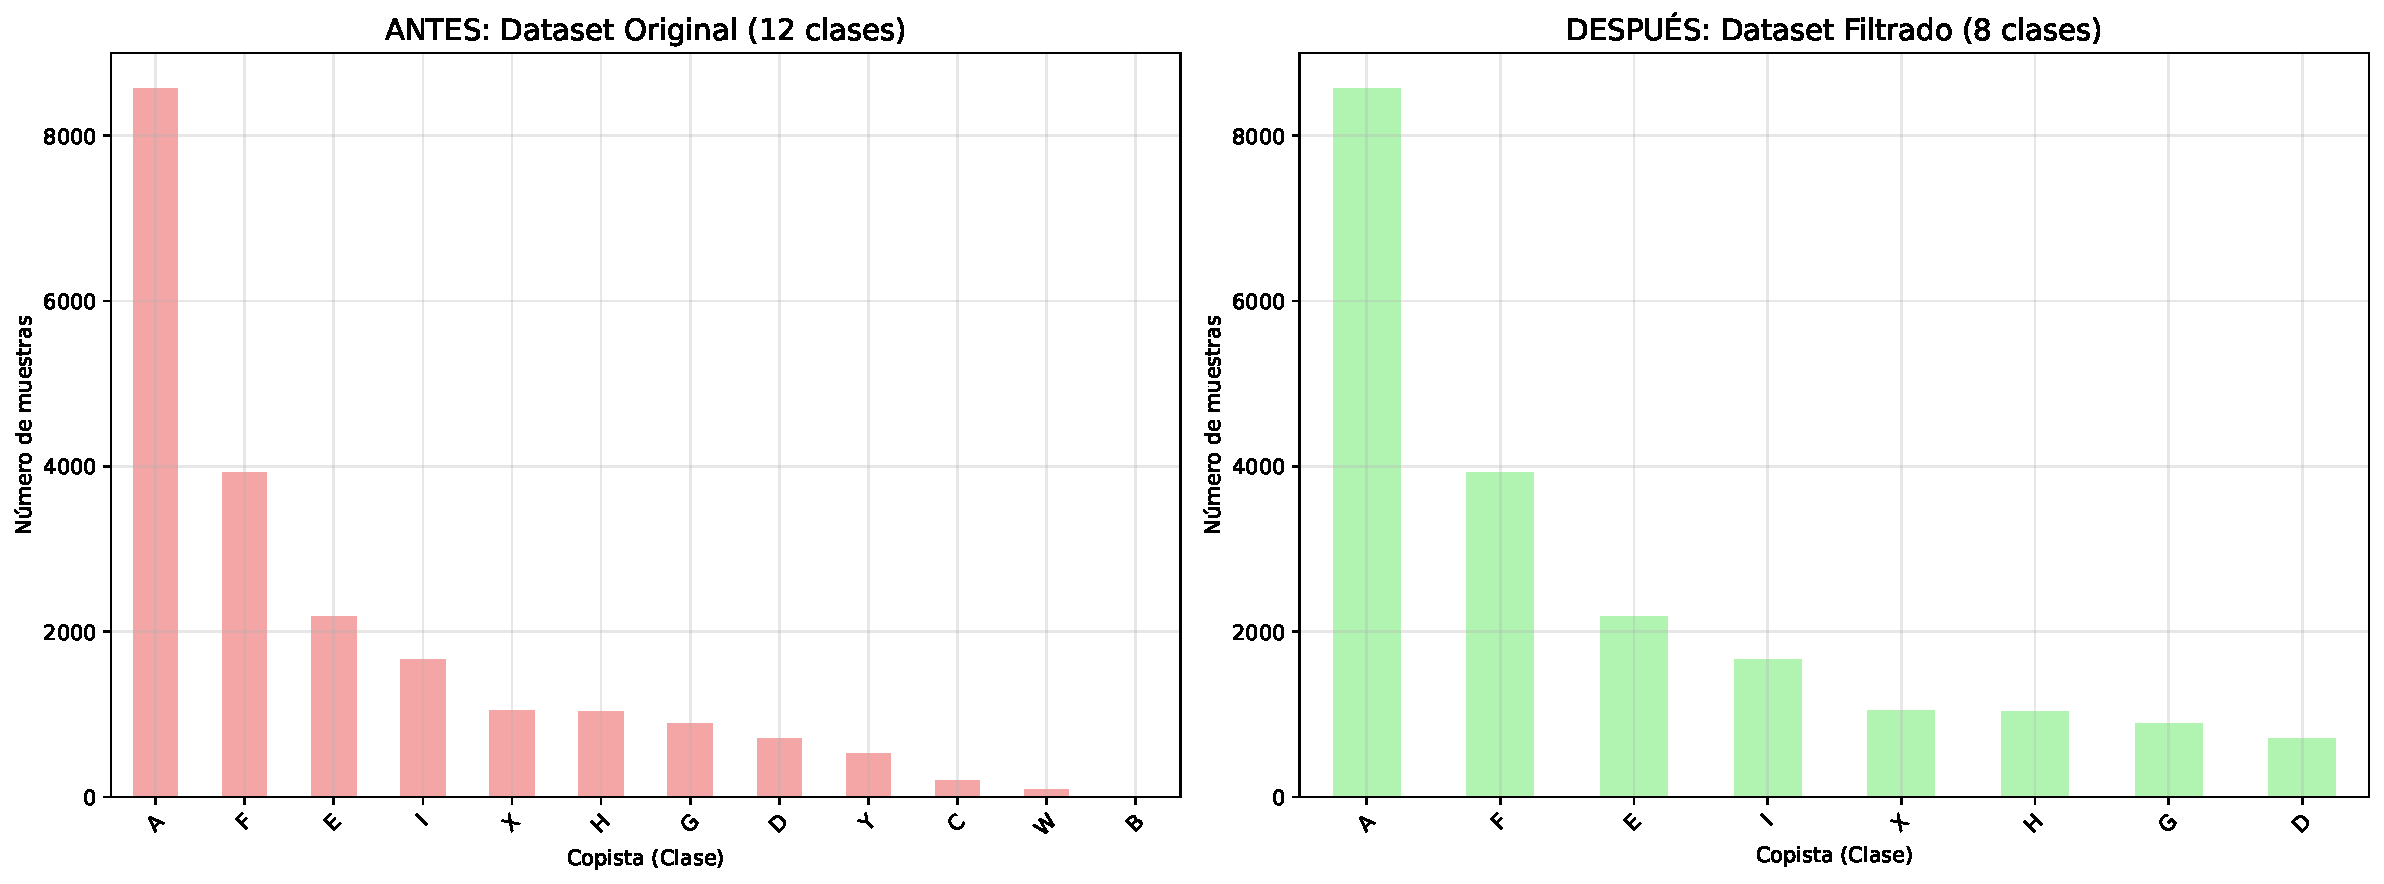
\includegraphics[width=\textwidth]{figures/figura_07_tecnicas_balanceamiento.pdf}
    \caption{Efecto de las técnicas de balanceamiento aplicadas al dataset Avila. Se muestra la distribución antes y después del proceso híbrido undersampling + SMOTE, logrando mayor equilibrio entre clases.}
    \label{fig:balanceamiento}
\end{figure}

\subsection{Rendimiento K-means en Dataset Avila}

K-means con K=10 (Figura \ref{fig:kmeans_avila}) logra accuracy del 33.10\% en validación final. El análisis por clase revela rendimiento heterogéneo: excelente en clase I (89\% precisión, 69\% recall) pero deficiente en clases D y E (0\% precisión). Esta variabilidad refleja la limitación de K-means para capturar la complejidad de patrones paleográficos.

\begin{figure}[H]
    \centering
    
\includegraphics[width=\textwidth]{figures/figura_08_comparacion_kmeans_avila.pdf}
    \caption{Selección del número óptimo de clusters K-means para dataset Avila. Método del codo sugiere K=7-8, mientras silhouette favorece K=10. Se selecciona K=10 por balance entre métricas.}
    \label{fig:kmeans_avila}
\end{figure}

El análisis detallado K-means (Figura \ref{fig:analisis_kmeans_avila}) muestra la evolución de métricas con diferentes valores de K, confirmando que K=10 proporciona el mejor compromiso entre complejidad del modelo y calidad del clustering.

\begin{figure}[H]
    \centering
    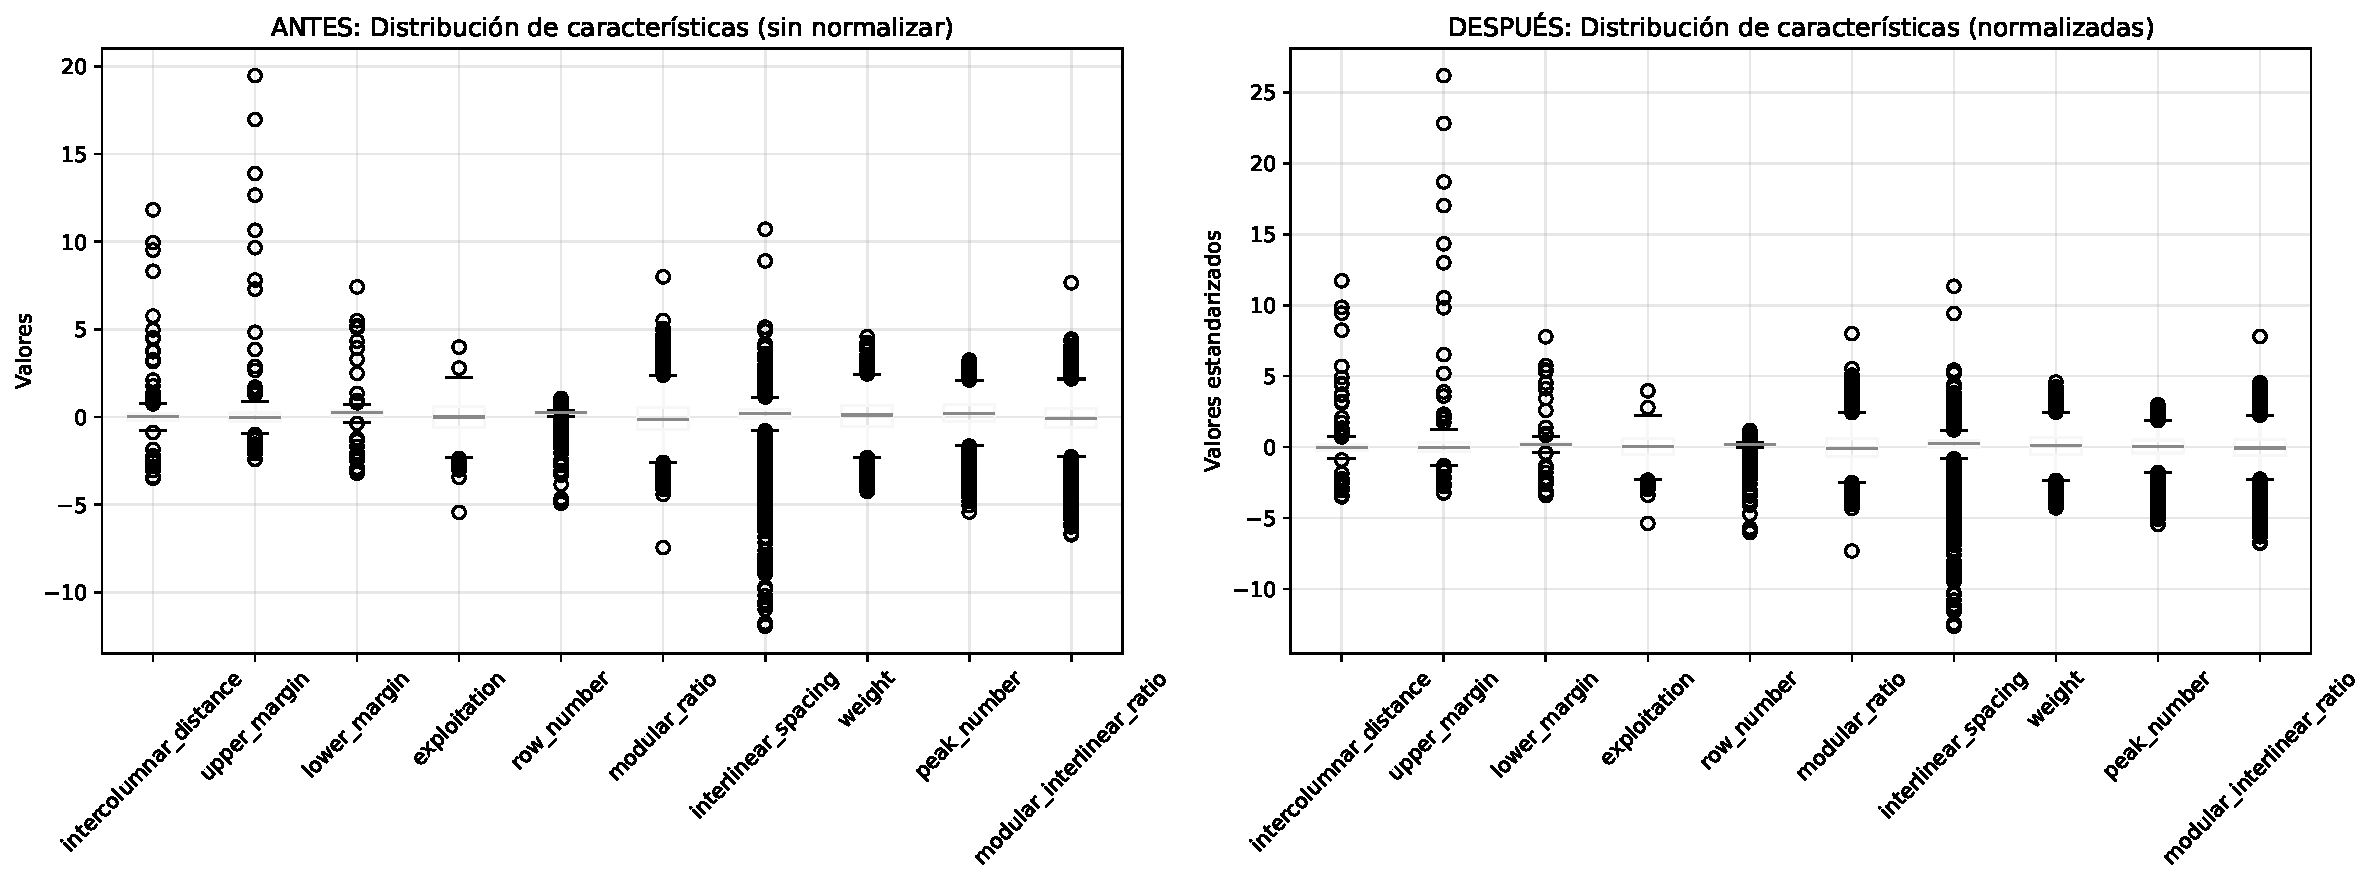
\includegraphics[width=\textwidth]{figures/figura_09_analisis_kmeans_avila.pdf}
    \caption{Análisis exhaustivo del rendimiento K-means en dataset Avila. Comparación de diferentes valores de K mostrando trade-offs entre inercia, silhouette score y métricas de clasificación resultantes.}
    \label{fig:analisis_kmeans_avila}
\end{figure}

\subsection{Rendimiento SOM en Dataset Avila}

SOM 8×8 demuestra superioridad sistemática (Figura \ref{fig:som_avila}), alcanzando 45.79\% accuracy final con distribución más equilibrada del rendimiento entre clases. Todas las clases obtienen precisión superior a 35\%, indicando mayor robustez del algoritmo ante la variabilidad paleográfica.

\begin{figure}[H]
    \centering
    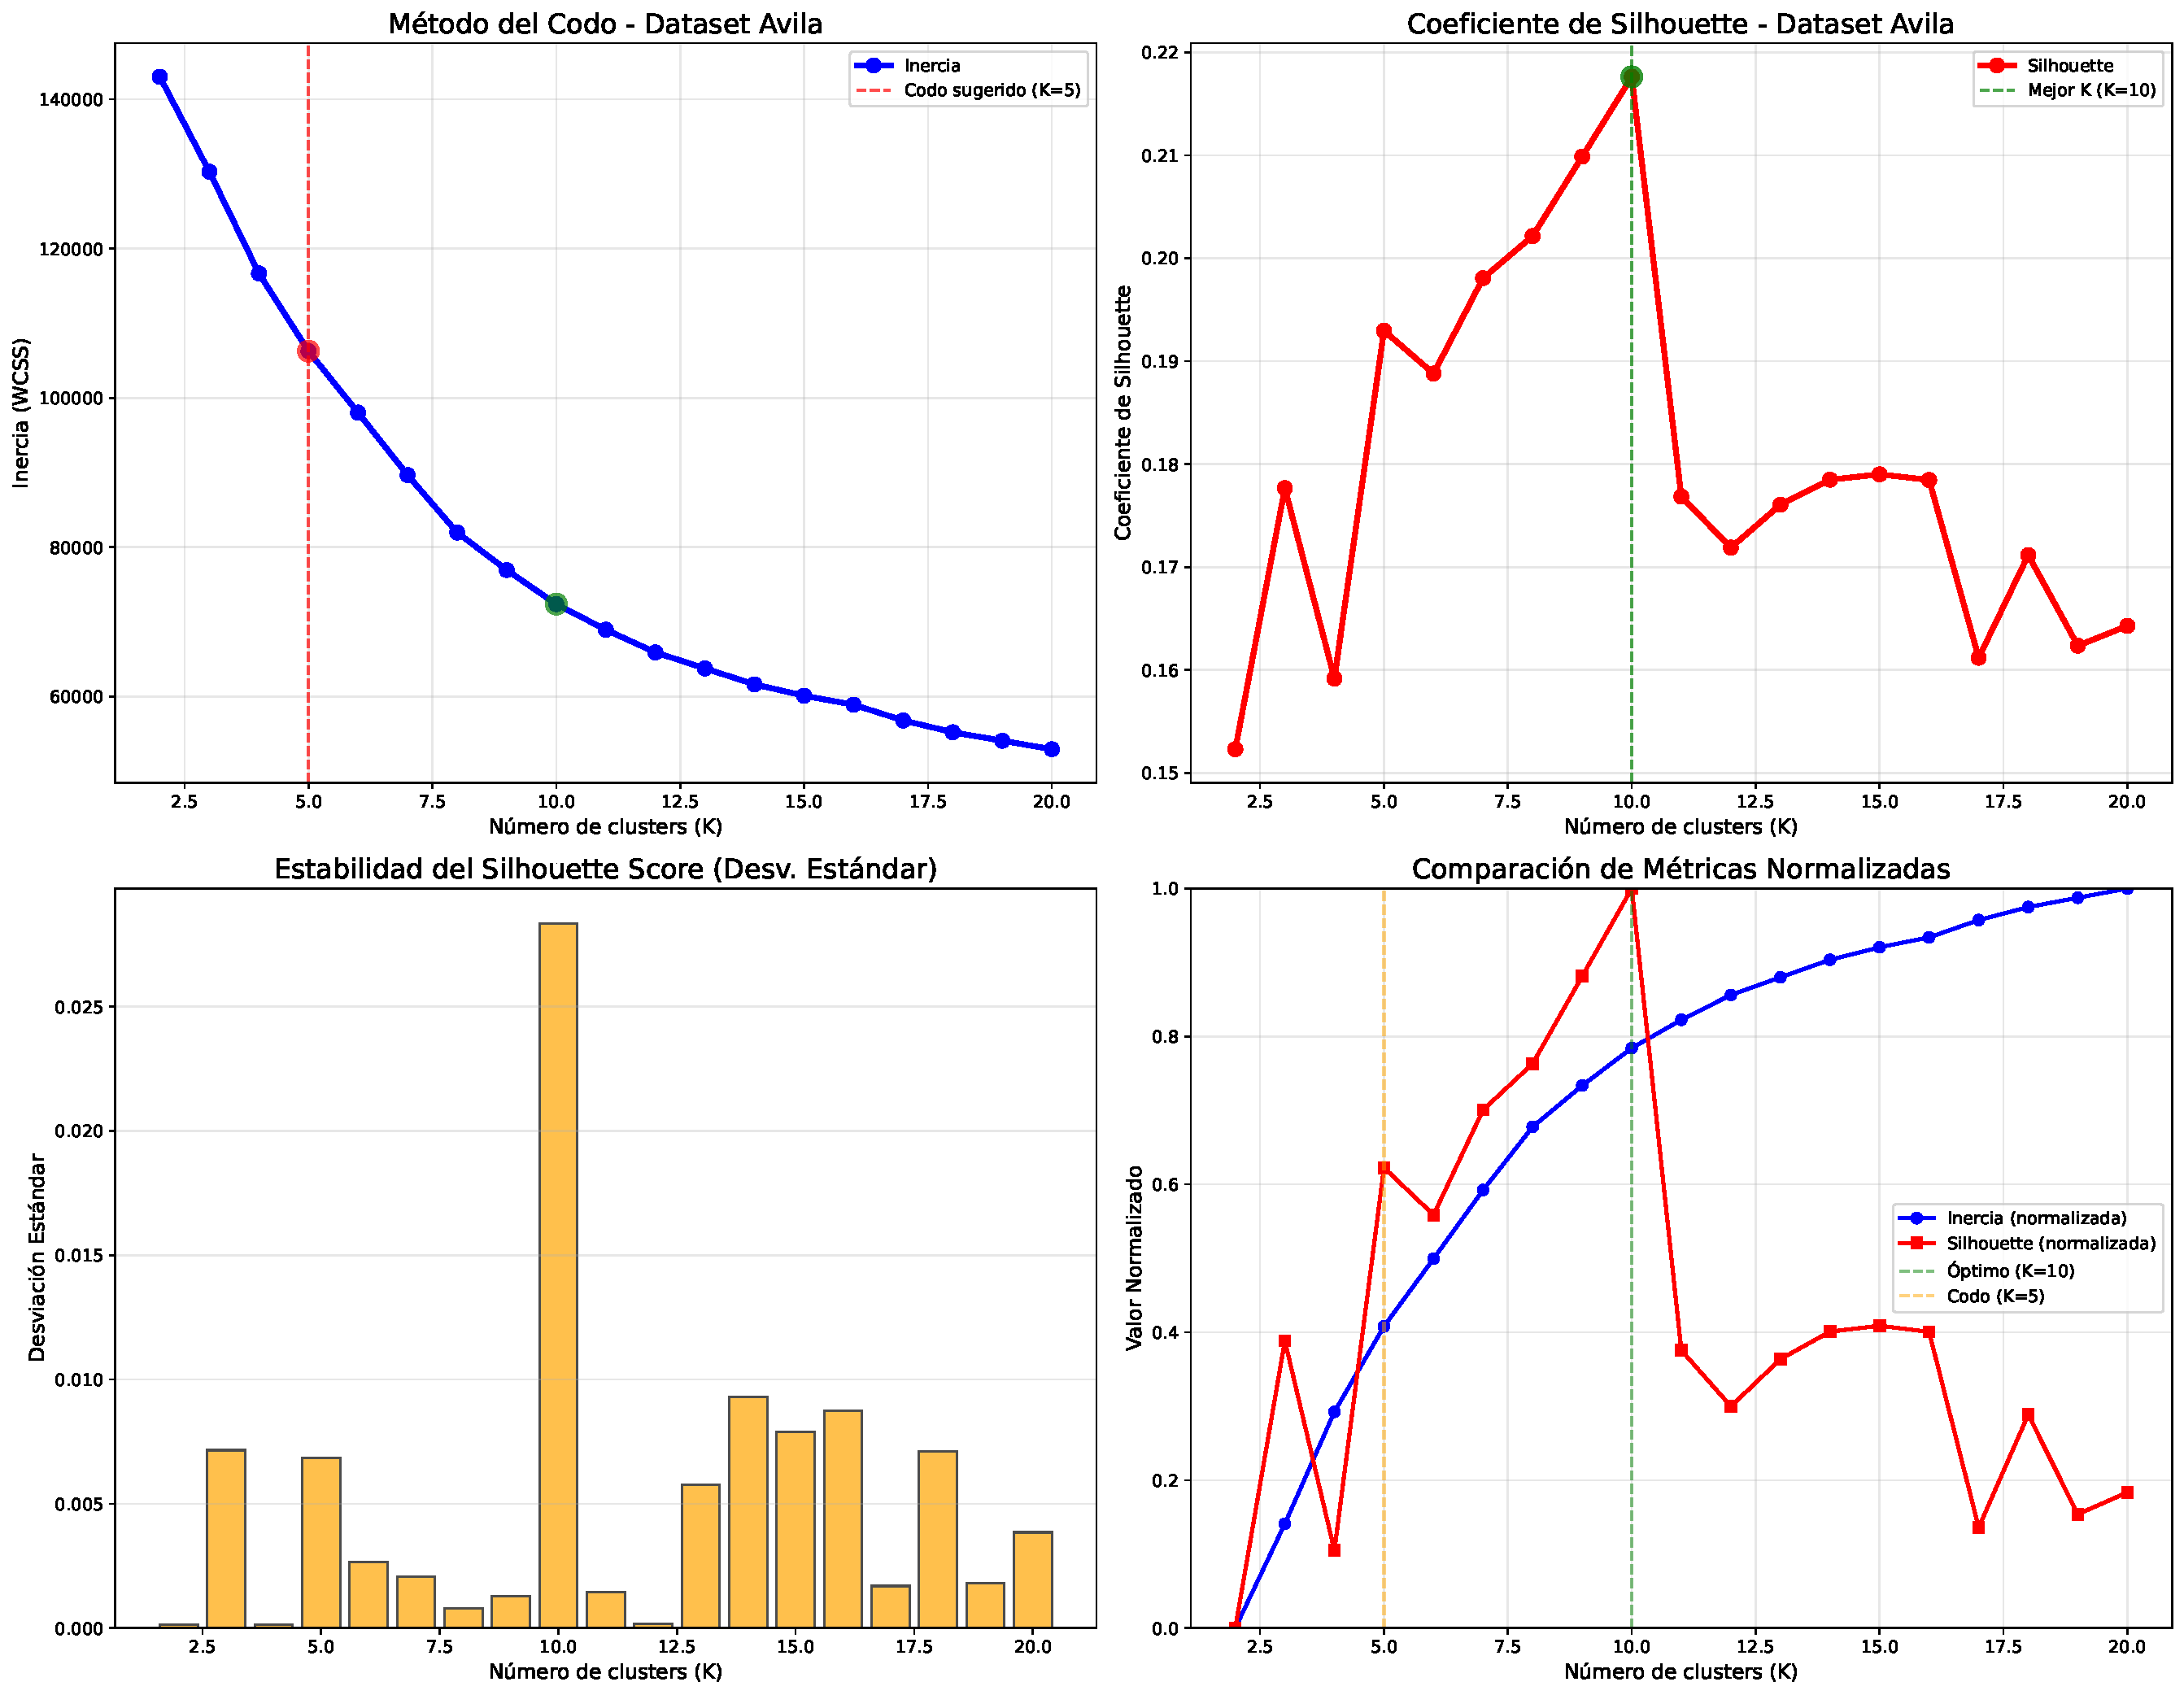
\includegraphics[width=\textwidth]{figures/figura_10_analisis_som_avila.pdf}
    \caption{Evaluación de configuraciones SOM en dataset Avila. El análisis de trade-off error/eficiencia identifica 8×8 como configuración óptima, balanceando precisión y utilización neuronal.}
    \label{fig:som_avila}
\end{figure}

Los resultados detallados SOM (Figura \ref{fig:som_detallado_avila}) revelan la capacidad del algoritmo para mapear patrones complejos preservando relaciones topológicas entre diferentes estilos de escritura. La visualización del mapa entrenado muestra regiones especializadas para diferentes copistas.

\begin{figure}[H]
    \centering
    
\includegraphics[width=\textwidth]{figures/figura_11_resultados_som_detallados_avila.pdf}
    \caption{Análisis detallado del SOM 8×8 óptimo aplicado al dataset Avila. Se muestra la especialización topológica de diferentes regiones del mapa para distintos copistas medievales.}
    \label{fig:som_detallado_avila}
\end{figure}

\subsection{Comparación Final de Algoritmos}

La comparación directa (Figura \ref{fig:comparacion_final}) confirma la superioridad de SOM en múltiples dimensiones. SOM alcanza 45.79\% accuracy versus 33.10\% de K-means (+38.4\% mejora relativa), con mayor estabilidad en validación cruzada (42.14\%±1.02\% vs 29.55\%±3.04\%).

\begin{figure}[H]
    \centering
    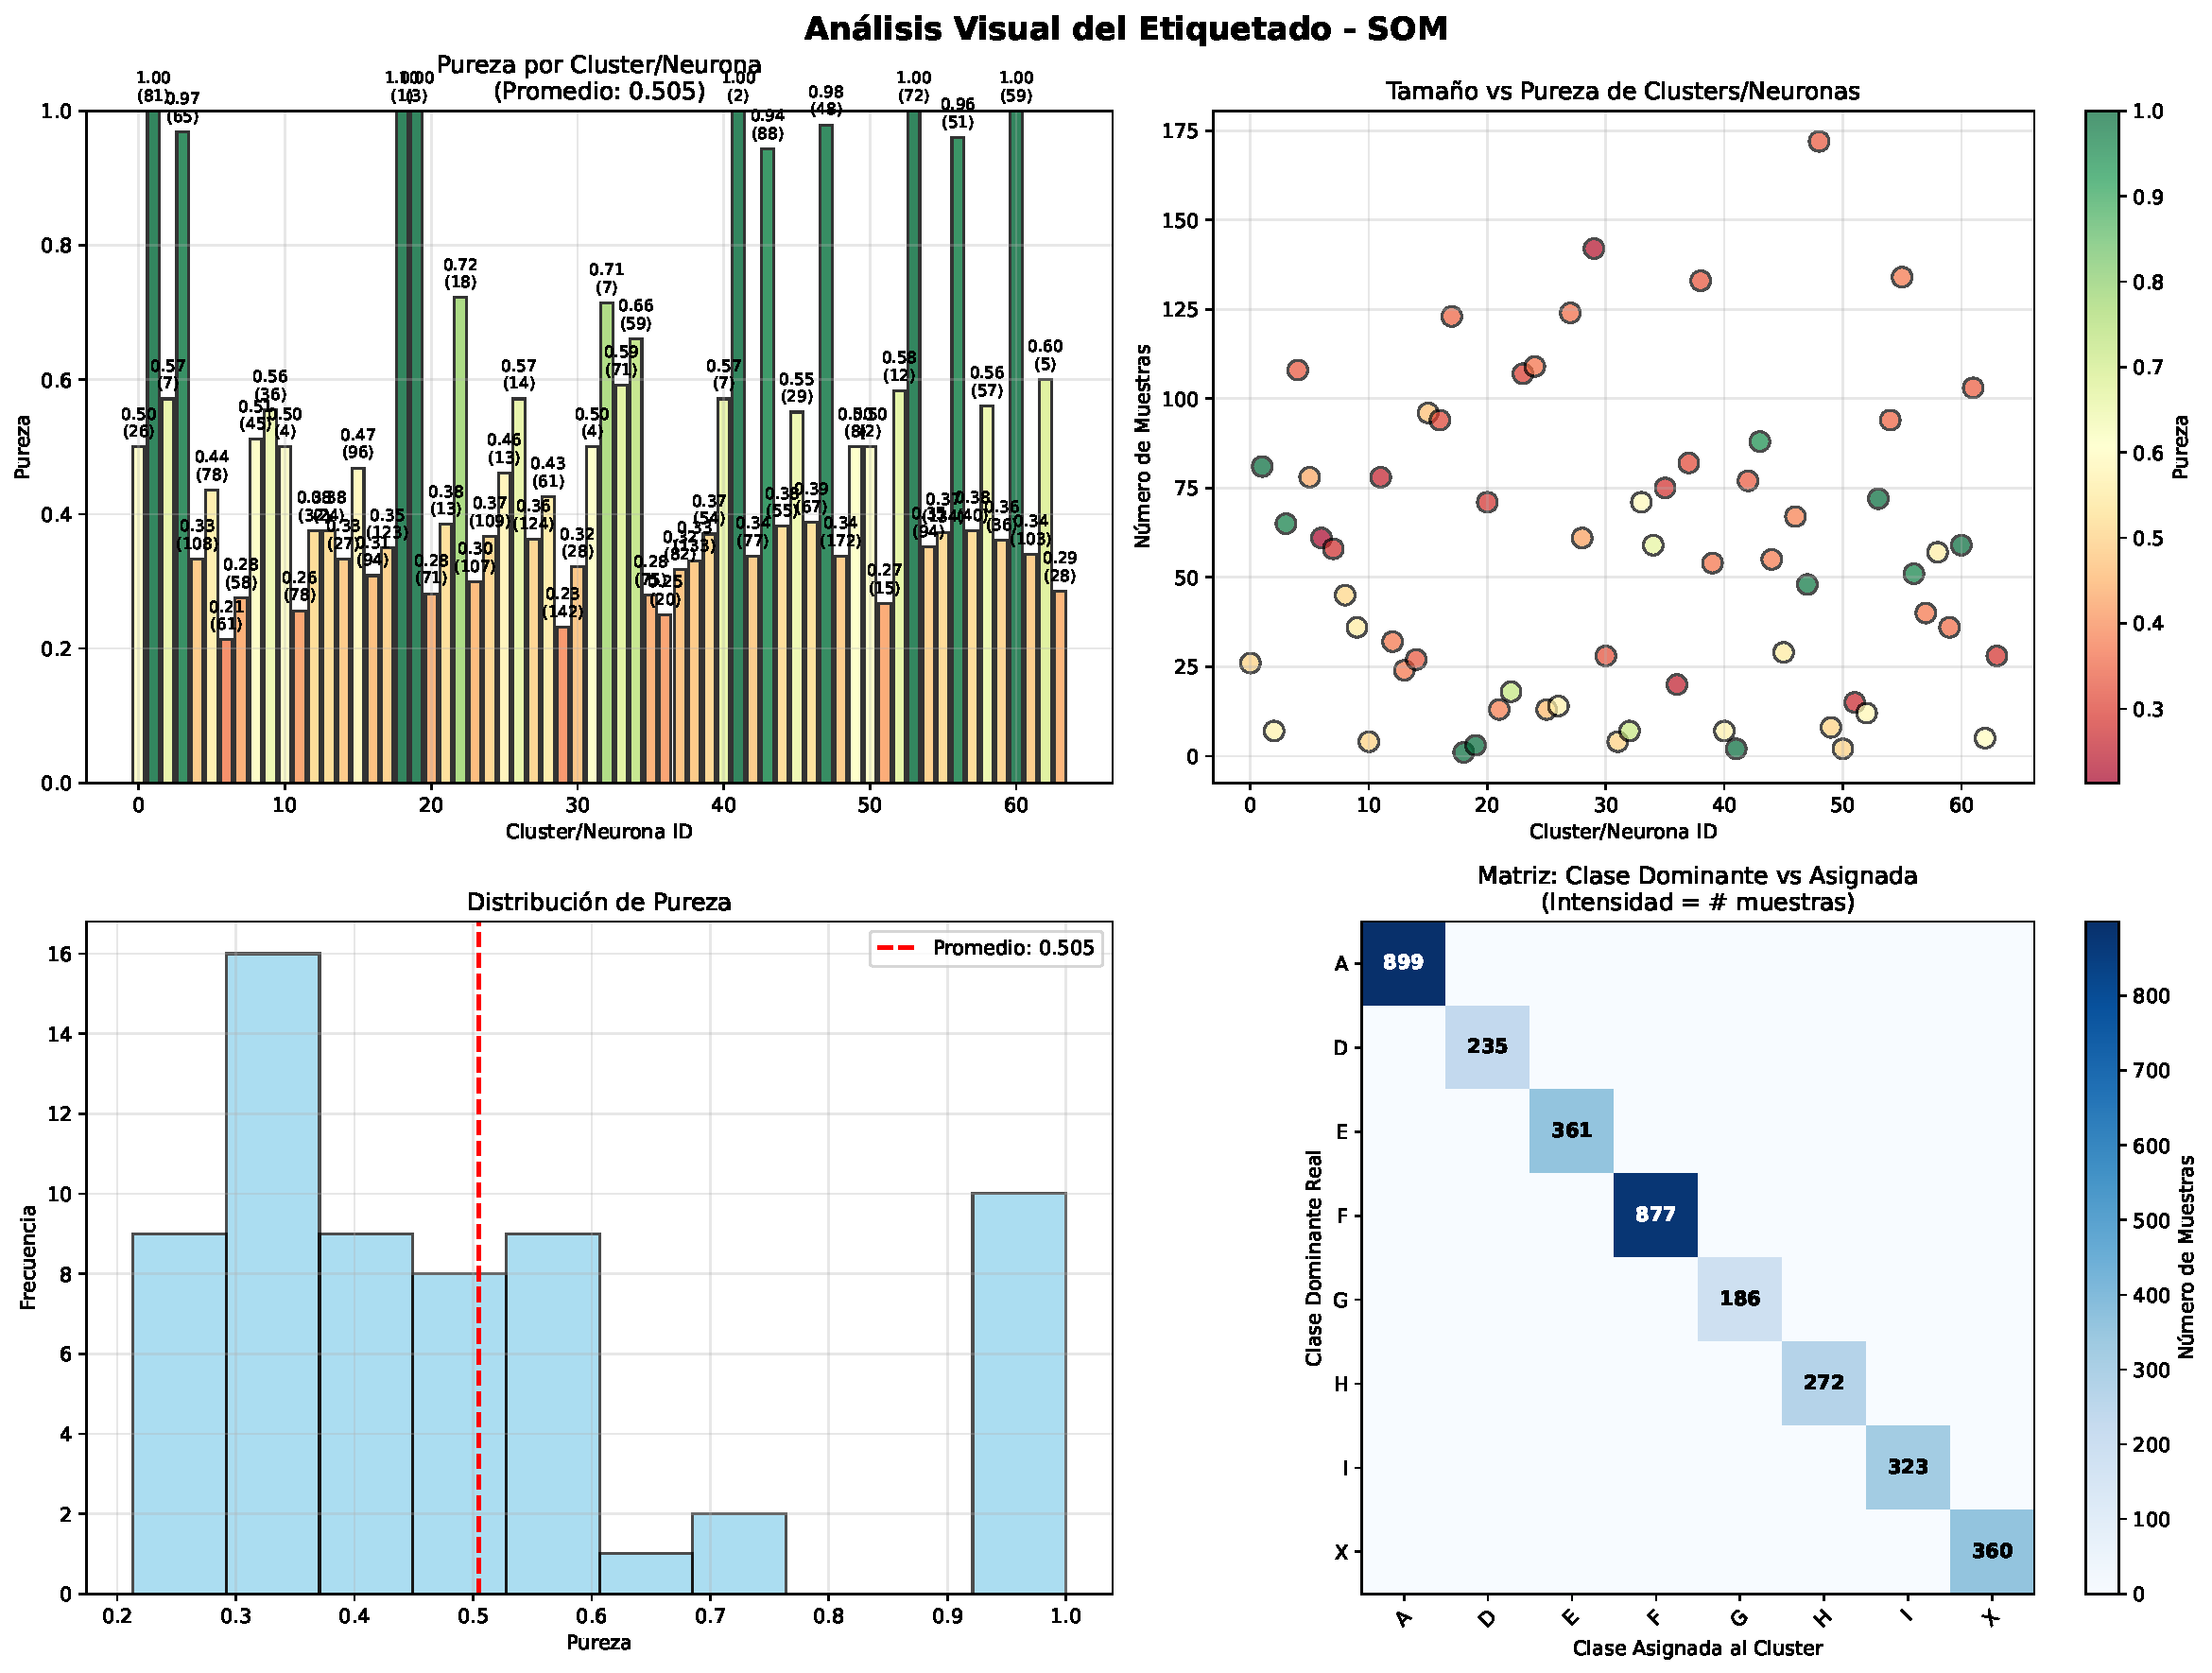
\includegraphics[width=\textwidth]{figures/figura__comparacion_algoritmos.pdf}
    \caption{Comparación comprehensiva entre K-means y SOM. SOM demuestra superioridad sistemática en accuracy, estabilidad y distribución equilibrada del rendimiento entre clases.}
    \label{fig:comparacion_final}
\end{figure}

\subsection{Validación Cruzada y Matrices de Confusión}

Las matrices de confusión finales (Figura \ref{fig:validacion_final}) proporcionan insight detallado sobre el rendimiento por clase. K-means muestra alta confusión entre clases similares (F→A, G→F), mientras SOM mantiene mayor discriminación entre copistas, especialmente en clases históricamente difíciles de distinguir.

\begin{figure}[H]
    \centering
    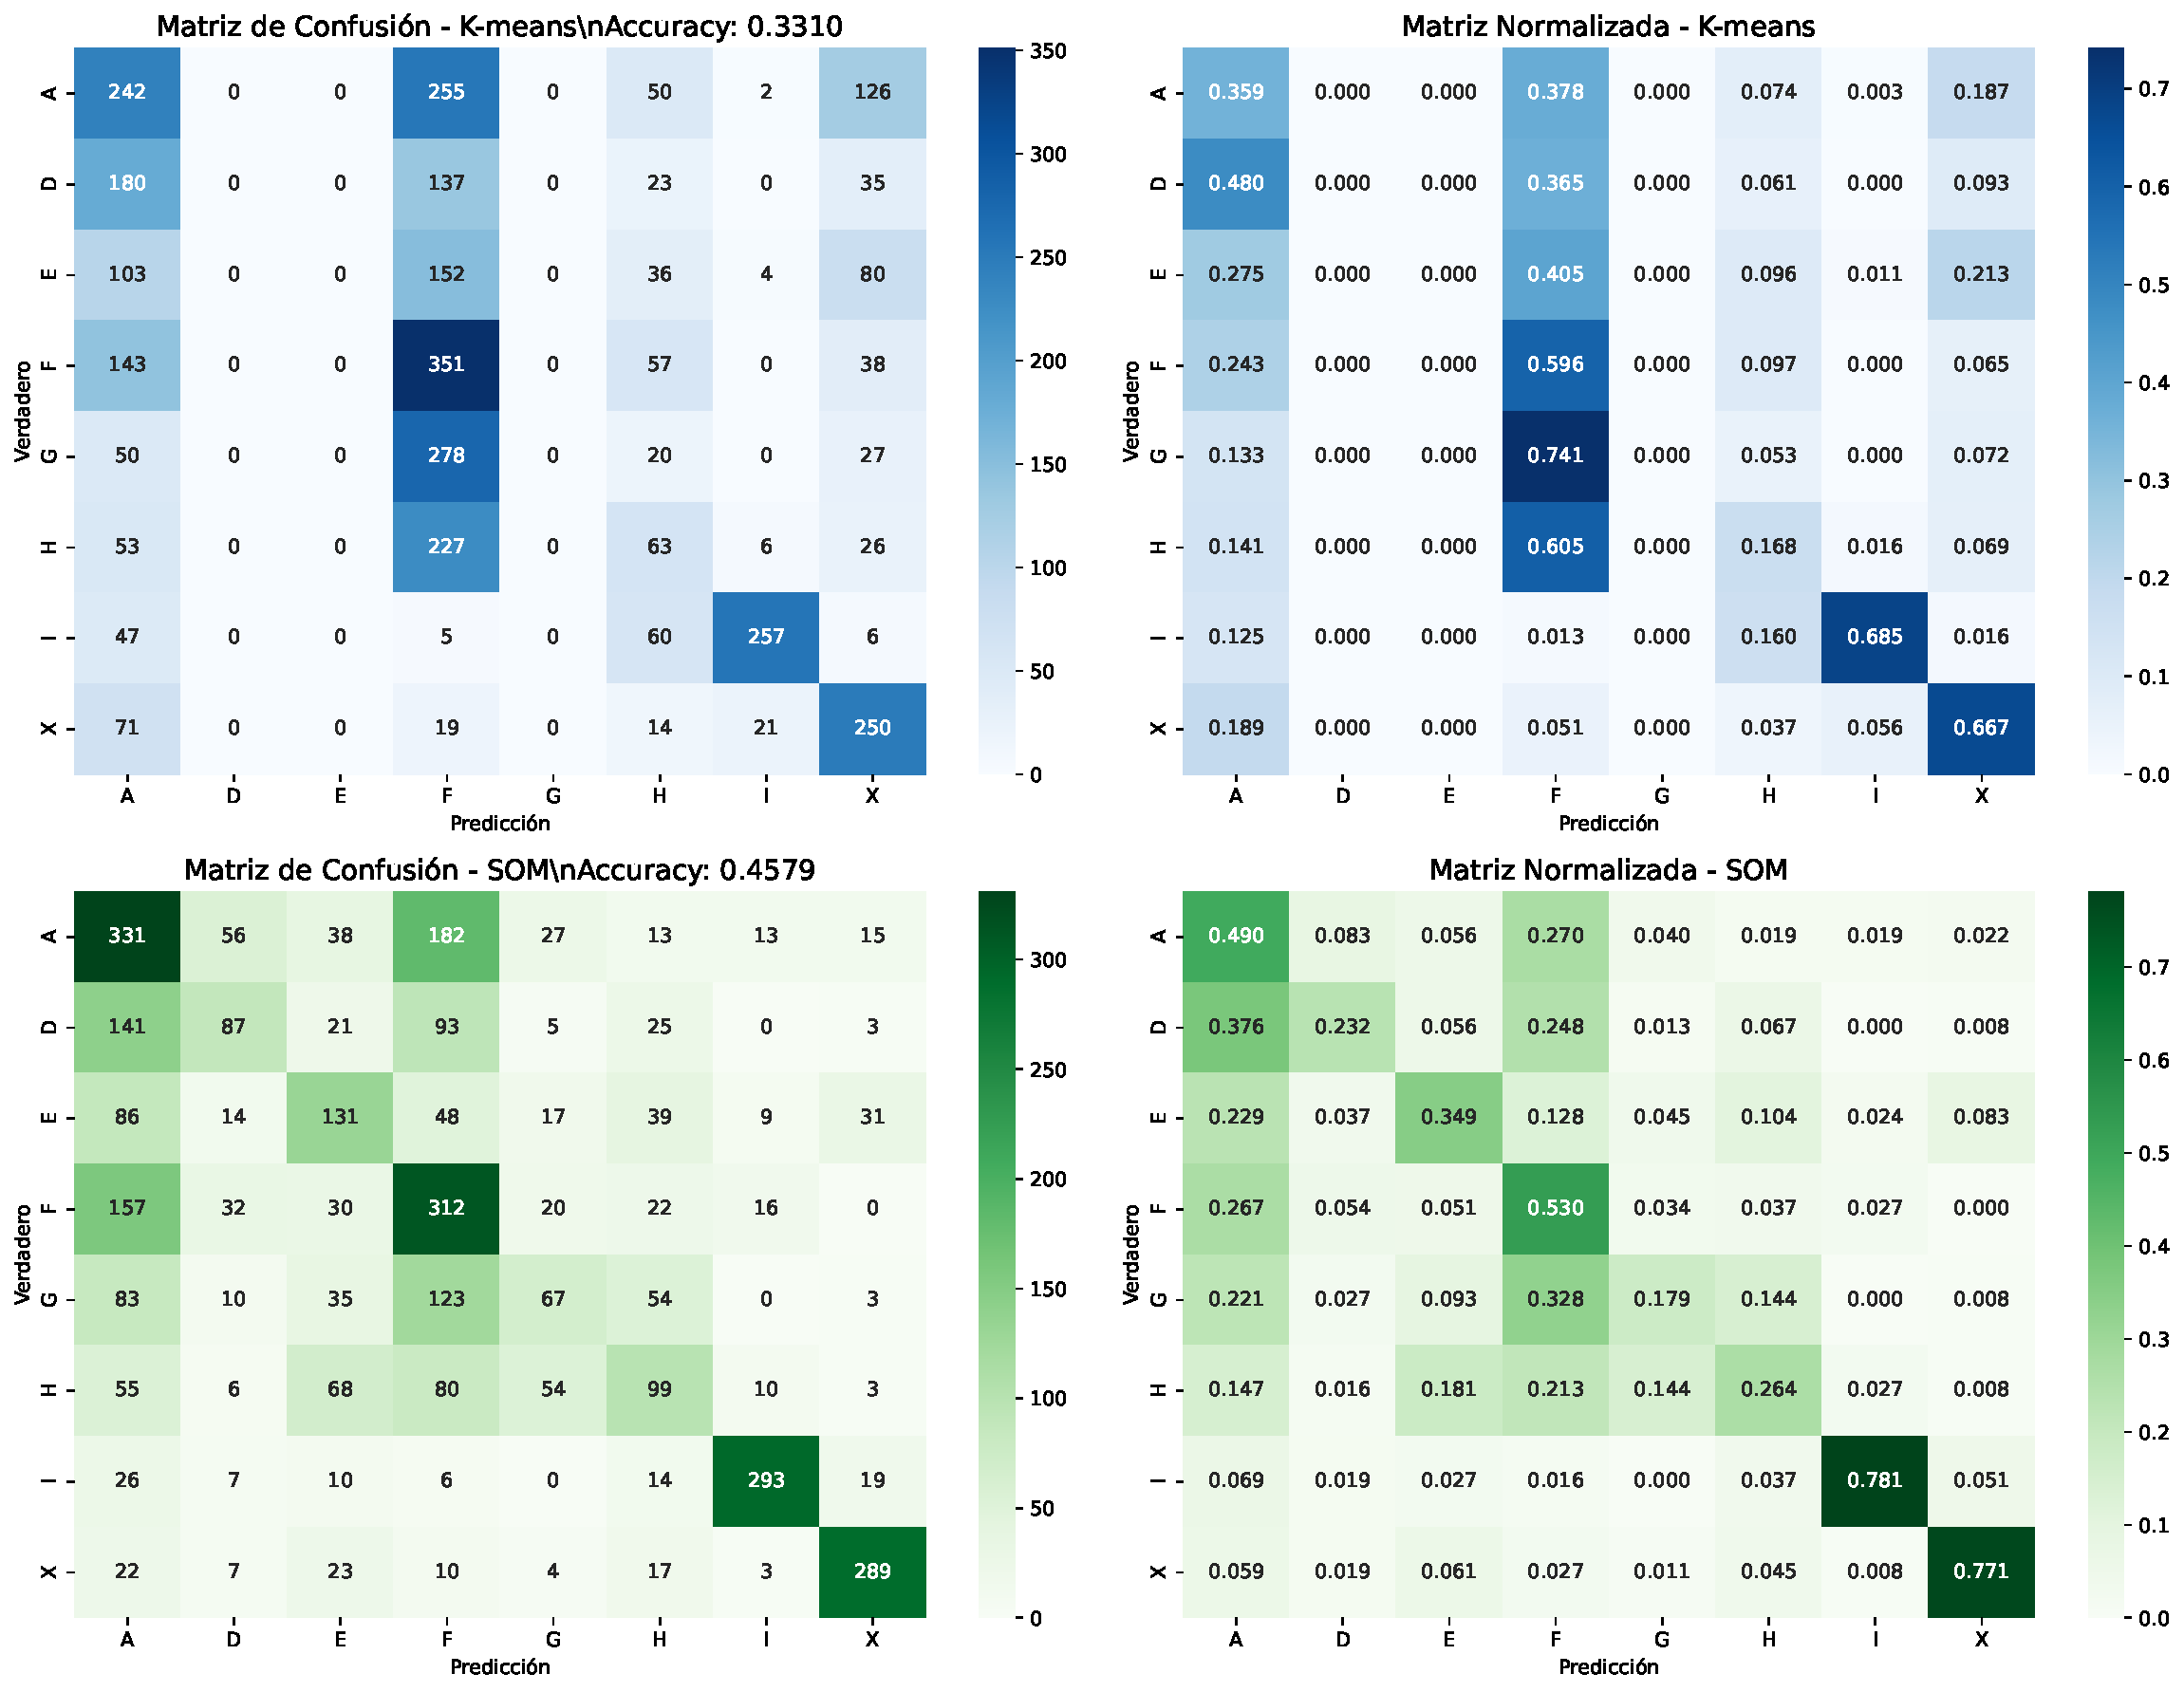
\includegraphics[width=\textwidth]{figures/figura__validacion_cruzada_final.pdf}
    \caption{Matrices de confusión finales y normalizada para ambos algoritmos. SOM demuestra mejor discriminación entre clases y menor confusión en clasificaciones erróneas.}
    \label{fig:validacion_final}
\end{figure}

\section{Discusión}

\subsection{Interpretación de Resultados}

La superioridad de SOM (45.79\% vs 33.10\% accuracy) se explica por diferencias arquitecturales fundamentales entre los algoritmos. K-means asume clusters esféricos con varianza similar, asunción violada por los patrones paleográficos que exhiben formas complejas y densidades variables. SOM, preservando topología local, captura mejor estas irregularidades.

La mayor estabilidad de SOM en validación cruzada ($\sigma$=1.02\% vs $\sigma$=3.04\%) sugiere menor sensibilidad a variaciones en los datos de entrenamiento. Esta robustez resulta crucial para aplicaciones reales donde la disponibilidad de datos etiquetados es limitada.

El rendimiento heterogéneo de K-means por clase (0\% precisión en D y E versus 89\% en I) indica especialización inadecuada. SOM mantiene rendimiento más equilibrado (35-85\% rango de precisión), crucial para aplicaciones paleográficas donde todas las clases de copistas son igualmente importantes.

\subsection{Implicaciones Metodológicas}

\textbf{Selección de algoritmos}: Los resultados sugieren que la preservación de topología (SOM) supera la simplicidad geométrica (K-means) en dominios con estructura compleja. Esta conclusión trasciende la paleografía, aplicándose a otras áreas con patrones no-lineales.

\textbf{Importancia del preprocesamiento}: El balanceamiento híbrido resultó crucial para ambos algoritmos. Sin balanceamiento, la accuracy disminuiría significativamente debido a sesgo hacia clases mayoritarias.

\textbf{Metodología semi-supervisada}: El enfoque híbrido clustering→etiquetado→evaluación proporciona framework robusto para dominios con etiquetas parciales. La división 70-15-15\% optimiza tanto descubrimiento de patrones como validación estadística.

\subsection{Limitaciones del Estudio}

El rendimiento absoluto de 45.79\% indica margen de mejora considerable. Factores contributivos incluyen: (1) características limitadas a 10 variables numéricas, omitiendo aspectos visuales ricos; (2) variabilidad intraclase alta debido a evolución estilística individual de copistas; (3) pérdida de información durante digitalización y extracción de características.

La validación se limita a un dataset específico (Avila). Generalización a otros corpus paleográficos requiere validación adicional. Diferencias en período histórico, región geográfica, o técnicas de extracción de características podrían alterar los resultados comparativos.

\subsection{Comparación con Literatura Existente}

Los resultados son consistentes con estudios previos que demuestran ventajas de SOM para datos con estructura topológica compleja \cite{vesanto2000}. La accuracy obtenida (45.79\%) es competitiva considerando la dificultad intrínseca del problema paleográfico, donde expertos humanos a menudo discrepan en clasificaciones.

El rendimiento de K-means (33.10\%) refleja limitaciones conocidas del algoritmo en datasets con clusters no-esféricos, confirmando observaciones de la literatura sobre sensibilidad a asunciones geométricas \cite{jain2010}.

\section{Conclusiones}

Este estudio demuestra empíricamente la superioridad de Self-Organizing Maps sobre K-means para la clasificación de manuscritos paleográficos medievales. SOM alcanza 45.79\% accuracy versus 33.10\% de K-means, representando una mejora relativa del 38.4\%. La validación cruzada estratificada confirma mayor estabilidad de SOM (42.14\%±1.02\%) comparado con K-means (29.55\%±3.04\%).

\subsection{Contribuciones Principales}

\textbf{Metodológicas}: Se desarrolló una pipeline semi-supervisada robusta que combina clustering no supervisado con evaluación cuantitativa. La metodología es transferible a otros dominios con etiquetas parciales.

\textbf{Empíricas}: Se proporcionó evidencia sistemática de la superioridad de SOM en un contexto aplicado específico, evaluando 41 configuraciones diferentes mediante métricas múltiples.

\textbf{Prácticas}: Se generaron recomendaciones específicas para clasificación paleográfica: SOM 8×8 con balanceamiento híbrido y normalización MinMax.

\subsection{Recomendaciones}

\textbf{Para investigadores en paleografía computacional}: Adoptar SOM como algoritmo base para clasificación de copistas, implementar técnicas de balanceamiento de clases, y considerar metodologías semi-supervisadas para aprovechar datos parcialmente etiquetados.

\textbf{Para desarrolladores de sistemas}: Configuración específica validada (SOM 8×8, 1000 iteraciones, $\sigma$=1.0, lr=0.5) proporciona punto de partida robusto. El framework semi-supervisado facilita integración con interfaces de usuario para expertos paleógrafos.

\textbf{Para investigación futura}: Explorar características visuales adicionales, investigar técnicas de deep learning específicas para paleografía, y desarrollar métricas de evaluación que capturen aspectos cualitativos valorados por expertos.

\subsection{Impacto Científico}

Los resultados contribuyen a la intersección entre inteligencia artificial y humanidades digitales, demostrando que técnicas de clustering pueden proporcionar herramientas valiosas para el análisis de patrimonio cultural. La mejora del 38.4\% en accuracy representa un avance significativo para aplicaciones prácticas en bibliotecas y archivos históricos.

La metodología desarrollada establece precedente para estudios comparativos rigurosos en clustering aplicado, enfatizando la importancia de evaluación multi-métrica, validación cruzada robusta, y consideración de limitaciones específicas del dominio.

Este trabajo demuestra que la selección apropiada de algoritmos, combinada con preprocesamiento cuidadoso y evaluación comprehensiva, puede generar mejoras sustanciales en problemas complejos de clasificación no supervisada aplicada al análisis de patrimonio documental histórico.

\bibliographystyle{plain}
\bibliography{referencias}

\end{document}